\documentclass{beamer}
\usepackage[serbian]{babel}
\usepackage[Serbian-Latn]{babel}

\setbeamersize{text margin left=5mm,text margin right=5mm}

%% tikz block diagrams %%
\usepackage{tikz}
\usetikzlibrary{arrows,positioning,shapes.geometric}
\usetikzlibrary{fit}
\usetikzlibrary{calc}
\usetikzlibrary{decorations.markings}
\usetikzlibrary{arrows.meta}
\usetikzlibrary{automata}

\usepackage[utf8]{inputenc}
\usetheme{Antibes}
% \usetheme{Berkeley}
% \usetheme{JuanLesPins}
% \usetheme{Warsaw}
\usepackage[]{graphicx}


\title[] %optional
{Hardverska implementacija Viola-Jones algoritma}

\subtitle{Diplomski rad}

\author[Risto Pejašinović]
{Risto Pejašinović}

\institute[FTN] % % (optional)
{
  Fakultet Tehničkih Nauka,
  Univerzitet u Novom Sadu
}

\date[Oktobar 2019] % (optional)
{Oktobar 2019}

\begin{document}
\frame{\titlepage}

\begin{frame}
  \frametitle{Sadržaj}
  \tableofcontents
\end{frame}

\section{Viola-Jones}

\subsection{Uvod}
\begin{frame}
  \frametitle{Viola-Jones Algoritam}
  Algoritam za detekciju objekata na slici.
  \begin{itemize}
  \item Paul Viola, Michael Jones 2001.
  \item<1-> Najčešće korišćen za detekciju lica.
  \item<1-> Mobilni telefoni, digitalni fotoaparati.
  \end{itemize}
\end{frame}

\begin{frame}
  \frametitle{Viola-Jones Algoritam}
  Tri ključne stvari.
  \begin{itemize}
  \item<1-> Integralna slika.
  \item<1-> AdaBoost.
  \item<1-> Kaskadni Klasifikator.
  \end{itemize}
\end{frame}

\subsection{Integralna slika}
% \begin{frame}
%   \frametitle{Integralna slika}
%   \begin{itemize}
%   \item<1-> Zaslužna za brzinu.
%   \item<1-> Jednostavna transformacija.
%   \item<1-> Računanje bilo koje površine u konstantnom vremenu.
%   \end{itemize}
% \end{frame}

\begin{frame}
  \frametitle{Integralna slika}
  Piksel integralne slike predstavlja zbir svih piksela koji se nalaze gore i levo
  na originalnoj slici.
  \begin{figure}[H]
    \centering
    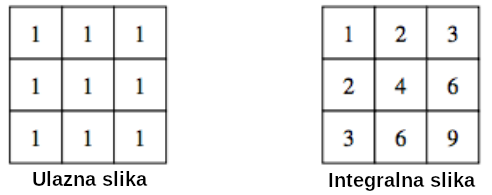
\includegraphics[width=0.55\linewidth]{../images/integral_image1}
  \end{figure}
\end{frame}

\begin{frame}
  \frametitle{Integralna slika}
  Računanje bilo koje površine u konstantnom vremenu. \\
  2 oduzimanja i jedno sabiranje.
  Potrebne samo ivice.
  \begin{figure}[H]
    \centering
    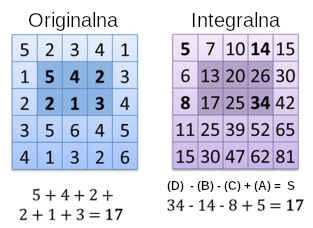
\includegraphics[width=0.55\linewidth]{../images/integral_image2}
  \end{figure}
\end{frame}

\subsection{HAAR obležja}
\begin{frame}{HAAR obeležja}
    \begin{columns}[onlytextwidth,T]
      \column{\dimexpr\linewidth-50mm-0mm}

      \begin{itemize}
      \item<1-> Ciljaju karakteristike objekta
      \item<1-> Pravougaona obeležja.
      \item<1-> 2 ili 3 pravougaonika i težina.
      \item<1-> Tipične dimenzije prozora 24x24.
      \item<1-> Oko 160,000 mogućih obeležja.
      \end{itemize}

      \column{60mm}

      \begin{figure}[H]
        \centering
        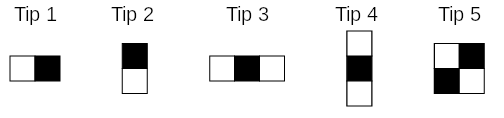
\includegraphics[width=0.8\linewidth]{../images/haar_features1}
      \end{figure}
    \end{columns}
\end{frame}

\begin{frame}
  \frametitle{HAAR obeležja, Ciljaju karakteristike objekta}
  Čelo svetlije od očiju. \\
  Nos svetliji od očiju. \\
  \begin{figure}[H]
    \centering
    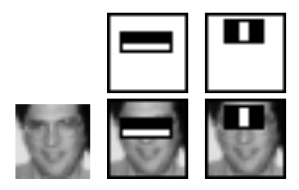
\includegraphics[width=0.7\linewidth]{../images/haar_features2}
  \end{figure}
\end{frame}


\subsection{Ada Boost}
\begin{frame}
  \frametitle{Ada Boost}

  \begin{itemize}
  \item<1-> Mašinsko učenje.
  \item<1-> 160,000 obeležja.
  \item<1-> Ponavljaju se, nisu sva korisna.
  \item<1-> Weak Learner 50\% +
  \item<1-> Kombinacijom Strong Classifier
  \end{itemize}

\end{frame}

\subsection{Kaskadni Klasifikator}
\begin{frame}
  \frametitle{Kaskadni Klasifikator}

  \begin{columns}[onlytextwidth,T]
    \column{\dimexpr\linewidth-60mm-2mm}
  \begin{itemize}
  \item<1-> 2913 obeležja u modelu.
  \item<1-> Veliki deo slike pozadina.
  \item<2-> Ranije odbacivanje pozadine.
  \item<2-> 2913 klasifikatora u 25 etapa.
  \item<3-> Posle pete etape odbačeno 99\%.
  \end{itemize}


  \column{80mm}
  \begin{overprint}
    \onslide<1>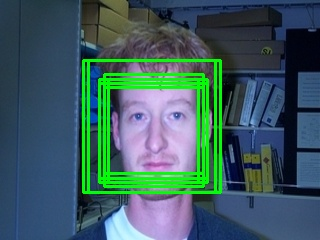
\includegraphics[width=0.7\linewidth]{../images/rotation_variance}
    \onslide<2>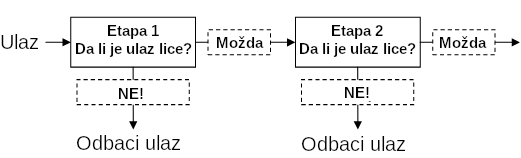
\includegraphics[width=0.9\linewidth]{../images/cascade_classifier1}
    \onslide<3>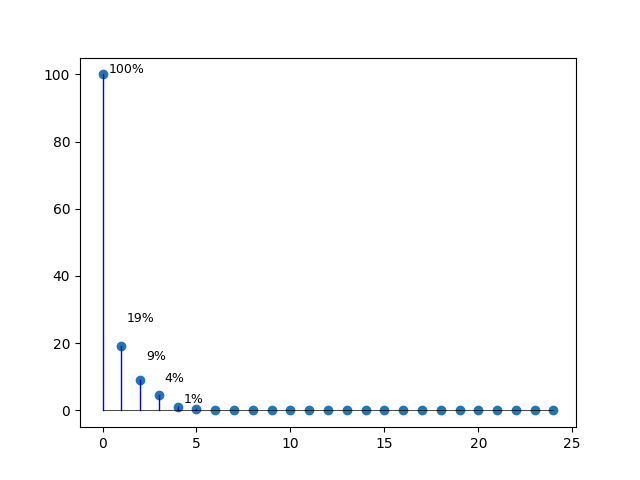
\includegraphics[width=0.9\linewidth]{../images/cascade_classifier2}
  \end{overprint}

  \end{columns}
\end{frame}

\subsection{Skaliranje slike}
\begin{frame}
  \frametitle{Skaliranje slike}

  \begin{columns}[onlytextwidth,T]
    \column{\dimexpr\linewidth-60mm-2mm}
    \begin{itemize}
    \item<1-> Objekti različite veličine.
    \item<2-> Piramida skaliranih slika.
    \end{itemize}


    \column{80mm}
    \begin{overprint}
      \onslide<1>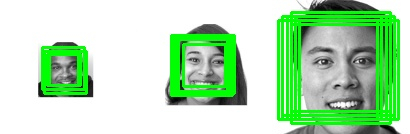
\includegraphics[width=0.83\linewidth]{../images/sixfaces_scaled_res}
      \onslide<2>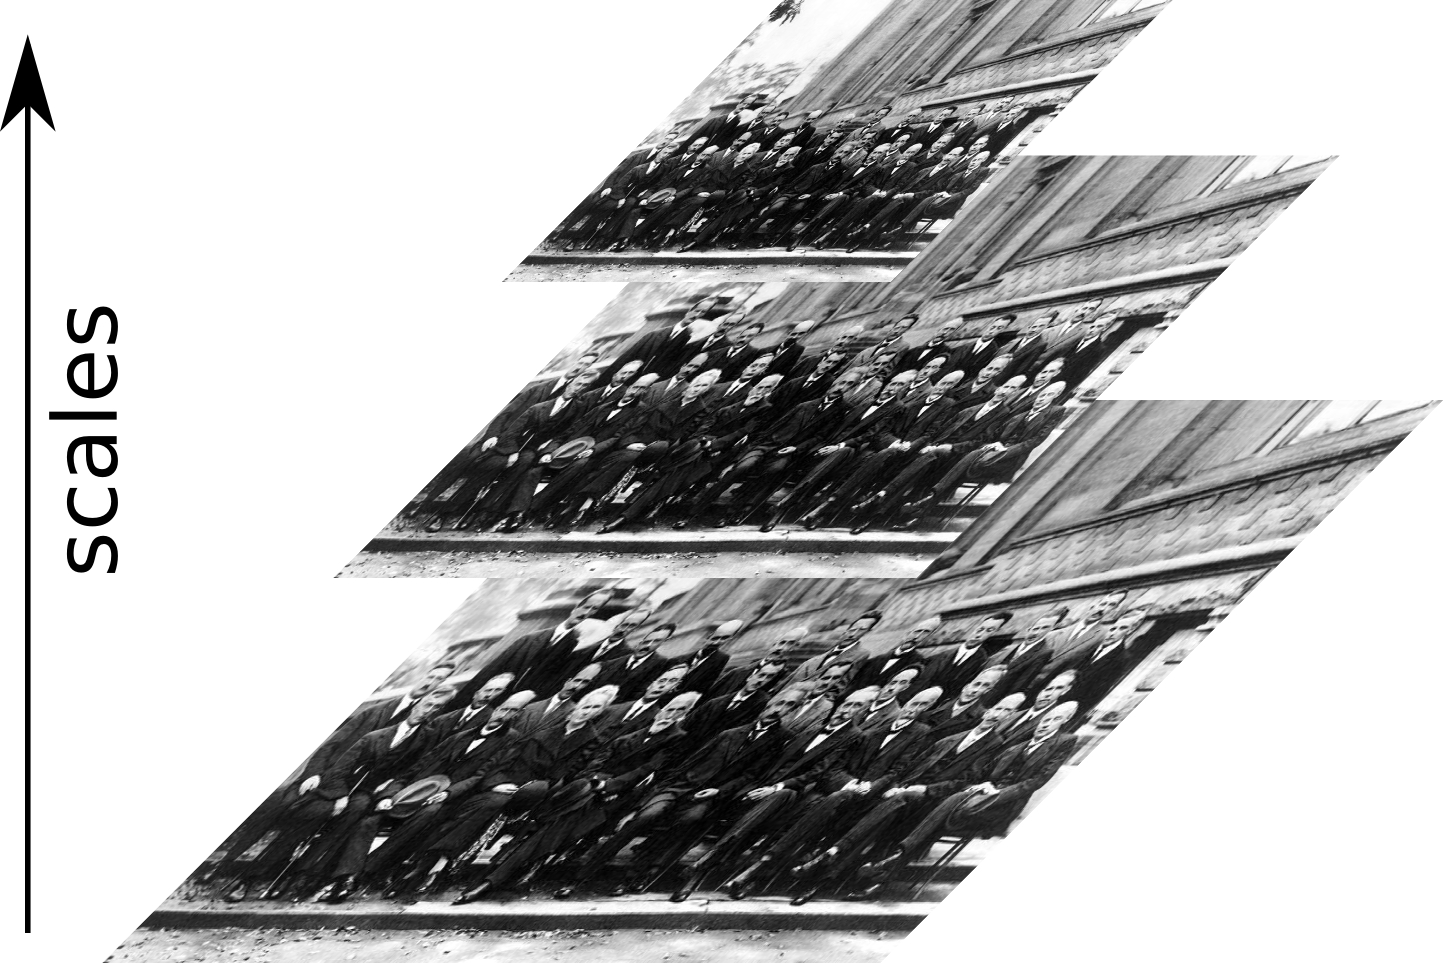
\includegraphics[width=0.7\linewidth]{../images/image_pyramid}
    \end{overprint}

  \end{columns}
\end{frame}

\subsection{Osetljivost na osvetljaj i rotaciju}
\begin{frame}
  \frametitle{Osetljivost na osvetljaj i rotaciju}

  \begin{columns}[onlytextwidth,T]
    \column{\dimexpr\linewidth-50mm-2mm}
    \begin{itemize}
    \item<1-> Osetljiv na osvetljaj.
    \item<2-> I na rotaciju.
    \end{itemize}


    \column{80mm}
    \begin{overprint}
      \onslide<1>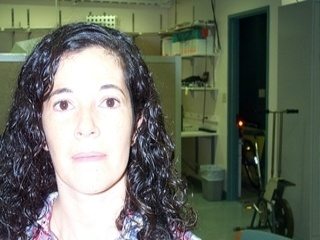
\includegraphics[width=0.7\linewidth]{../images/overexposed_light}
      \onslide<2>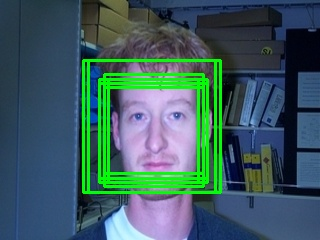
\includegraphics[width=0.7\linewidth]{../images/rotation_variance}
      \onslide<3>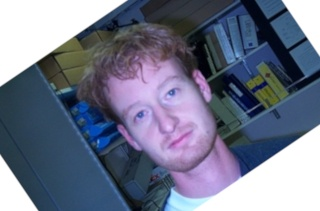
\includegraphics[width=0.7\linewidth]{../images/rotated_res}
    \end{overprint}

  \end{columns}
\end{frame}


\section{OpenCV}
\begin{frame}
  \frametitle{OpenCV}

  \begin{itemize}
  \item<1-> Istrenirani modeli (.xml fajl).
  \item<1-> Alat za treniranje.
  \item<1-> Implementacija klasifikatora.
  % \item<1-> Treba parsirati .xml fajl.
  % \item<1-> haarcascaade\_frontalface\_default.xml
  % \item<1-> Python za parsiranje.
  \end{itemize}

\end{frame}

\section{Specifikacije za izvršavanje}
\begin{frame}
  \frametitle{Specifikacije za izvršavanje}
  \begin{columns}[onlytextwidth,T]
    \column{\dimexpr\linewidth-55mm-2mm}
    \begin{itemize}
    \item<1-> Python XML parser.
    \item<1-> Python klasa klasifikatora.
    \item<1-> Python klasifikator.
    \item<1-> C++ Header model fajl.
    \item<1-> C++ klasifikator.
    \end{itemize}

    \column{80mm}
    \begin{overprint}
      \onslide<1>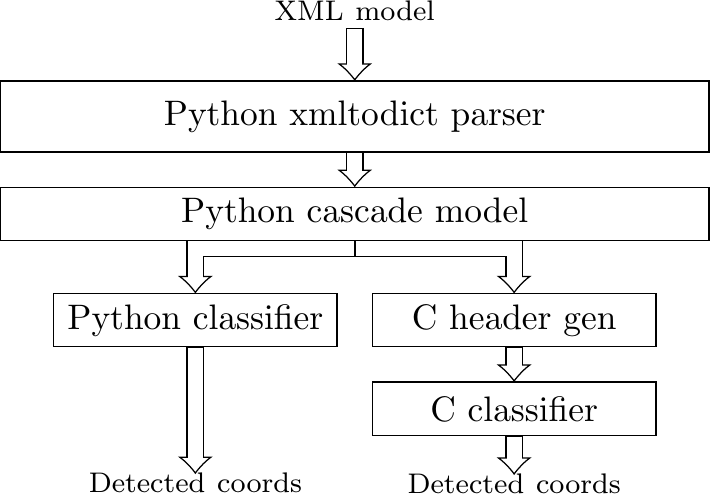
\includegraphics[width=0.77\linewidth]{../images/bdp/sw_arch/sw_arch1}
    \end{overprint}

  \end{columns}

\end{frame}


\section{Arhitektura hardvera}

\begin{frame}
  \frametitle{Arhitektura hardvera}
  \begin{figure}[H]
    \centering{
      \resizebox{1.00\textwidth}{!}{%
        \pgfdeclarelayer{background}
\pgfdeclarelayer{foreground}
\pgfsetlayers{background,main,foreground}

\tikzstyle{cloud1} = [draw=black, thick, fill=red!20, minimum hegiht = 1em]
\tikzstyle{block_l} =[draw, text centered, fill=blue!15, minimum width=3cm, minimum height=3.5cm]
\tikzstyle{block_m} =[draw, text centered, fill=blue!15, minimum width=2.5cm, minimum height=2cm]
\tikzstyle{block_s} =[draw, text centered, fill=blue!15, minimum width=2cm, minimum height=1.5cm]
\tikzstyle{line} = [draw, decoration={markings,mark=at position 1 with {\arrow[scale=2.2,black]{>}}},
    postaction={decorate},
    shorten >=0.4pt]

\begin{tikzpicture}[thick]
  \node [block_l] (img_ram) {IMG RAM};
  \node [coordinate, above = 0cm of img_ram, yshift=-0.5cm, xshift=1.5cm] (img_ram_addr_in){};
  \node [coordinate, left =2.0cm of img_ram] (img_in){};
  \node [coordinate, left = 0cm of img_ram] (img_ram_img_in){};
  \node [coordinate, right = 0cm of img_ram] (img_ram_img_out){};

  \node [block_m, above right = +1cm and 0.2cm of img_ram] (rd_addrgen) {rd\_addrgen};
  \node [coordinate, below = 0cm of rd_addrgen] (rd_addr_addr_out){};

  \node [block_m, above right = -1.75cm and 2.5cm of img_ram ] (ii_gen) {ii\_gen};
  \node [coordinate, left = 0cm of ii_gen] (ii_gen_in){};
  \node [coordinate, right = 0cm of ii_gen] (ii_gen_out){};
  \node [block_m, below = 0.25cm of ii_gen ] (sii_gen) {sii\_gen};
  \node [coordinate, left = 0cm of sii_gen] (sii_gen_in){};
  \node [coordinate, right = 0cm of sii_gen] (sii_gen_out){};

  \node [block_s, right = 1.25cm of sii_gen ] (stddev) {stddev};
  \node [coordinate, above left = -0.25cm and 0cm of stddev] (stddev_ii){};
  \node [coordinate, above left = -0.75cm and 0cm of stddev] (stddev_sii){};
  \node [coordinate, right = 0cm of stddev] (stddev_out){};

  \node [block_m, right = 1.0cm of ii_gen ] (frame_buffer) {frame\_buffer};
  \node [coordinate, left = 0cm of frame_buffer] (frame_buffer_in){};
  \node [coordinate, above left = -0.5cm and 0cm of frame_buffer] (frame_buffer_rect_addr){};
  \node [coordinate, right = 0cm of frame_buffer] (frame_buffer_out){};

  \node [block_m, above = 1.0cm of frame_buffer ] (features_mem) {features\_mem};
  \node [coordinate, left = 0cm of features_mem] (rects_addr){};
  \node [coordinate, right = 0cm of features_mem] (rects_weights){};

  \node [block_l, fill=red!15, above right = -3.5cm and 1cm of frame_buffer] (classifier) {\huge Classifier};
  \node [coordinate, above left = -1cm and 0cm of classifier] (classifier_ii){};
  \node [coordinate, above left = -2.5cm and 0cm of classifier] (classifier_stddev){};
  \node [coordinate, above left = -0.5cm and 0cm of classifier] (classifier_weights){};
  \node [coordinate, above right = -1.0cm and 0cm of classifier] (detected_addr){};
  \node [coordinate, above right = -2.5cm and 0cm of classifier] (irq){};

  %% group %%
 \begin{pgfonlayer}{background}
  \node[inner sep=7pt, fill=yellow!25, rounded corners, inner ysep =30pt, draw, thick,fit=(img_ram) (rd_addrgen) (ii_gen) (features_mem) (sii_gen) (frame_buffer) (stddev) (classifier)] (ip_core) {};
  \node[above left] at (ip_core.south east) {\huge Cascade Classifier IP core};
\end{pgfonlayer}

  % arrows
  \path [line] (rd_addr_addr_out)  |- (img_ram_addr_in) node[transition, xshift=0.8cm, yshift=0.25cm] {rd\_addr};
  \path [line] (img_in) node[transition, yshift=0.25cm, xshift=0.65cm]{\large img\_in} -- (img_ram_img_in);
  \path [line] (img_ram_img_out) node[transition, yshift=0.2cm, xshift=0.9cm] {img\_out} -- +(1.75cm, 0cm) |- (ii_gen_in);
  \path [line] (img_ram_img_out) -- +(1.75cm, 0cm) |- (sii_gen_in);
  \path [line] (ii_gen_out) -- +(0.5cm, 0cm) node[transition, yshift=0.2cm, xshift=0cm] {ii} |- (stddev_ii);
  \path [line] (sii_gen_out) -- +(0.5cm, 0cm)  node[transition, yshift=0.2cm, xshift=0cm] {sii} |- (stddev_sii);
  \path [line] (ii_gen_out) |- (frame_buffer);
  \path [line] (frame_buffer_out) node[transition, yshift=+0.2cm, xshift=0.5cm] {fb\_ii} |- (classifier_ii);
  \path [line] (stddev_out) -- +(0.5cm, 0) node[transition, yshift=-0.2cm, xshift=0.1cm] {stddev} |- (classifier_stddev);
  \path [line] (rects_addr) node[transition, yshift=+0.2cm, xshift=-1.1cm] {rects\_addr}  -- +(-0.5cm, 0cm) |- (frame_buffer_rect_addr);
  \path [line] (rects_weights) node[transition, yshift=+0.2cm, xshift=+1.2cm] {rects\_weights}  -- +(+0.5cm, 0cm) |- (classifier_weights);
  \path [line] (detected_addr) -- +(3.0cm, 0cm) node[transition, yshift=0.25cm, xshift=-1.1cm]{\large detect\_addr} ;
  \path [line] (irq) -- +(3.0cm, 0cm) node[transition, yshift=0.25cm, xshift=-0.4cm]{\large irq} ;
\end{tikzpicture}

      }}
  \end{figure}
\end{frame}

\begin{frame}
   \frametitle<1->{Interfejsi}
   \frametitle<2->{IMG RAM}

  \begin{itemize}
  \item<1-1> \textbf{img\_in} ulazna slika.
  \item<1-1> \textbf{detect\_addr} detektovane koordinate.
  \item<1-1> \textbf{irq} interapt signal, zavšetak slike.

  \item<2-2> RAM memorija, za skladištenje slike.
  \item<2-2> Ušteda pristupa eksternoj memoriji.
  \end{itemize}

  \begin{figure}[H]
    \centering{
      \resizebox{.87\textwidth}{!}{%
        \pgfdeclarelayer{background}
\pgfdeclarelayer{foreground}
\pgfsetlayers{background,main,foreground}

\tikzstyle{cloud1} = [draw=black, thick, fill=red!20, minimum hegiht = 1em]
\tikzstyle{block_l} =[draw, text centered, fill=blue!15, minimum width=3cm, minimum height=3.5cm]
\tikzstyle{block_m} =[draw, text centered, fill=blue!15, minimum width=2.5cm, minimum height=2cm]
\tikzstyle{block_s} =[draw, text centered, fill=blue!15, minimum width=2cm, minimum height=1.5cm]
\tikzstyle{line} = [draw, decoration={markings,mark=at position 1 with {\arrow[scale=2.2,black]{>}}},
    postaction={decorate},
    shorten >=0.4pt]

\begin{tikzpicture}[thick]
  \node [block_l] (img_ram) {IMG RAM};
  \node [coordinate, above = 0cm of img_ram, yshift=-0.5cm, xshift=1.5cm] (img_ram_addr_in){};
  \node [coordinate, left =2.0cm of img_ram] (img_in){};
  \node [coordinate, left = 0cm of img_ram] (img_ram_img_in){};
  \node [coordinate, right = 0cm of img_ram] (img_ram_img_out){};

  \node [block_m, above right = +1cm and 0.2cm of img_ram] (rd_addrgen) {rd\_addrgen};
  \node [coordinate, below = 0cm of rd_addrgen] (rd_addr_addr_out){};

  \node [block_m, above right = -1.75cm and 2.5cm of img_ram ] (ii_gen) {ii\_gen};
  \node [coordinate, left = 0cm of ii_gen] (ii_gen_in){};
  \node [coordinate, right = 0cm of ii_gen] (ii_gen_out){};
  \node [block_m, below = 0.25cm of ii_gen ] (sii_gen) {sii\_gen};
  \node [coordinate, left = 0cm of sii_gen] (sii_gen_in){};
  \node [coordinate, right = 0cm of sii_gen] (sii_gen_out){};

  \node [block_s, right = 1.25cm of sii_gen ] (stddev) {stddev};
  \node [coordinate, above left = -0.25cm and 0cm of stddev] (stddev_ii){};
  \node [coordinate, above left = -0.75cm and 0cm of stddev] (stddev_sii){};
  \node [coordinate, right = 0cm of stddev] (stddev_out){};

  \node [block_m, right = 1.0cm of ii_gen ] (frame_buffer) {frame\_buffer};
  \node [coordinate, left = 0cm of frame_buffer] (frame_buffer_in){};
  \node [coordinate, above left = -0.5cm and 0cm of frame_buffer] (frame_buffer_rect_addr){};
  \node [coordinate, right = 0cm of frame_buffer] (frame_buffer_out){};

  \node [block_m, above = 1.0cm of frame_buffer ] (features_mem) {features\_mem};
  \node [coordinate, left = 0cm of features_mem] (rects_addr){};
  \node [coordinate, right = 0cm of features_mem] (rects_weights){};

  \node [block_l, fill=red!15, above right = -3.5cm and 1cm of frame_buffer] (classifier) {\huge Classifier};
  \node [coordinate, above left = -1cm and 0cm of classifier] (classifier_ii){};
  \node [coordinate, above left = -2.5cm and 0cm of classifier] (classifier_stddev){};
  \node [coordinate, above left = -0.5cm and 0cm of classifier] (classifier_weights){};
  \node [coordinate, above right = -1.0cm and 0cm of classifier] (detected_addr){};
  \node [coordinate, above right = -2.5cm and 0cm of classifier] (irq){};

  %% group %%
 \begin{pgfonlayer}{background}
  \node[inner sep=7pt, fill=yellow!25, rounded corners, inner ysep =30pt, draw, thick,fit=(img_ram) (rd_addrgen) (ii_gen) (features_mem) (sii_gen) (frame_buffer) (stddev) (classifier)] (ip_core) {};
  \node[above left] at (ip_core.south east) {\huge Cascade Classifier IP core};
\end{pgfonlayer}

  % arrows
  \path [line] (rd_addr_addr_out)  |- (img_ram_addr_in) node[transition, xshift=0.8cm, yshift=0.25cm] {rd\_addr};
  \path [line] (img_in) node[transition, yshift=0.25cm, xshift=0.65cm]{\large img\_in} -- (img_ram_img_in);
  \path [line] (img_ram_img_out) node[transition, yshift=0.2cm, xshift=0.9cm] {img\_out} -- +(1.75cm, 0cm) |- (ii_gen_in);
  \path [line] (img_ram_img_out) -- +(1.75cm, 0cm) |- (sii_gen_in);
  \path [line] (ii_gen_out) -- +(0.5cm, 0cm) node[transition, yshift=0.2cm, xshift=0cm] {ii} |- (stddev_ii);
  \path [line] (sii_gen_out) -- +(0.5cm, 0cm)  node[transition, yshift=0.2cm, xshift=0cm] {sii} |- (stddev_sii);
  \path [line] (ii_gen_out) |- (frame_buffer);
  \path [line] (frame_buffer_out) node[transition, yshift=+0.2cm, xshift=0.5cm] {fb\_ii} |- (classifier_ii);
  \path [line] (stddev_out) -- +(0.5cm, 0) node[transition, yshift=-0.2cm, xshift=0.1cm] {stddev} |- (classifier_stddev);
  \path [line] (rects_addr) node[transition, yshift=+0.2cm, xshift=-1.1cm] {rects\_addr}  -- +(-0.5cm, 0cm) |- (frame_buffer_rect_addr);
  \path [line] (rects_weights) node[transition, yshift=+0.2cm, xshift=+1.2cm] {rects\_weights}  -- +(+0.5cm, 0cm) |- (classifier_weights);
  \path [line] (detected_addr) -- +(3.0cm, 0cm) node[transition, yshift=0.25cm, xshift=-1.1cm]{\large detect\_addr} ;
  \path [line] (irq) -- +(3.0cm, 0cm) node[transition, yshift=0.25cm, xshift=-0.4cm]{\large irq} ;
\end{tikzpicture}

      }}
  \end{figure}
\end{frame}

\subsection{rd\_addrgen}

\begin{frame}
  \frametitle<1->{rd\_addrgen}

  \begin{itemize}
  \item<1-2> Generiše adrese za čitanje iz IMG RAM.

  \end{itemize}

  \begin{figure}[H]
    \centering
    \resizebox{1.1\textwidth}{!}{%
      \centering{
      \begin{overprint}
        \onslide<1>
\pgfdeclarelayer{background}
\pgfdeclarelayer{foreground}
\pgfsetlayers{background,main,foreground}

\tikzstyle{cloud1} = [draw=black, thick, fill=red!20, minimum height = 1em]
\tikzstyle{block_l} =[draw, text centered, fill=red!15, minimum width=2.5cm, minimum height=2.5cm]
\tikzstyle{block_m} =[draw, text centered, fill=blue!15, minimum width=2.5cm, minimum height=1.5cm]
\tikzstyle{block_s} =[draw, text centered, fill=blue!15, minimum width=2cm, minimum height=1.5cm]
\tikzstyle{line} = [draw, thick, decoration={markings,mark=at position 1 with {\arrow[scale=2.2,black]{>}}},
    postaction={decorate},
    shorten >=0.4pt]
\tikzstyle{line_s} = [draw, ->]
\tikzstyle{line_st} = [draw,thick, ->]

\begin{tikzpicture}
  % draw the grid and the numbers
  \draw (-1,+1) grid (7,9) foreach \i in {0,...,7}{
    (\i-.5,9.5) node{\i} (-1.5,8.5-\i) node{\i}};

  % for every line we give first and last index to fill
  \foreach[count=\j] \a/\b in {0/4,0/4,0/4,0/4,0/4}
    \foreach \i in {\a,...,\b}
    \fill[blue!35,shift={(-.5,+9.5)},yscale=-1] (\i,\j) circle(2.0mm);

    \foreach \y in {8.5,...,5.5}{
      \foreach \x in {-0.5}{
        \path [line] (\x, \y) -- (\x+4, \y);
        \path [line_s] (\x+4, \y) -- (-.5, \y-1);%
      }}
    \path [line] (-0.5, 4.5) -- (-0.5+4, 4.5);
    \path [line_st] (+2.0, +10.0) node[transition, yshift=0.3cm, xshift=-0.5cm] {sweeper} -- (+2.0, 8.5);
    \path [line_st] (0.0, +10.0) node[transition, yshift=0.3cm, xshift=-0.5cm] {hopper} -- (-0.5, 8.5);

\end{tikzpicture}
        \onslide<2>\pgfdeclarelayer{background}
\pgfdeclarelayer{foreground}
\pgfsetlayers{background,main,foreground}

\tikzstyle{cloud1} = [draw=black, thick, fill=red!20, minimum height = 1em]
\tikzstyle{block_l} =[draw, text centered, fill=red!15, minimum width=2.5cm, minimum height=2.5cm]
\tikzstyle{block_m} =[draw, text centered, fill=blue!15, minimum width=2.5cm, minimum height=1.5cm]
\tikzstyle{block_s} =[draw, text centered, fill=blue!15, minimum width=2cm, minimum height=1.5cm]
\tikzstyle{line} = [draw, thick, decoration={markings,mark=at position 1 with {\arrow[scale=2.2,black]{>}}},
    postaction={decorate},
    shorten >=0.4pt]
\tikzstyle{line_s} = [draw, ->]
\tikzstyle{line_st} = [draw,thick, ->]

\begin{tikzpicture}
  % draw the grid and the numbers
  \draw (-1,+1) grid (7,9) foreach \i in {0,...,7}{
    (\i-.5,9.5) node{\i} (-1.5,8.5-\i) node{\i}};

  % for every line we give first and last index to fill
  \foreach[count=\j] \a/\b in {0/4,0/4,0/4,0/4,0/4}
    \foreach \i in {\a,...,\b}
    \fill[blue!35,shift={(+2.5,+9.5)},yscale=-1] (\i,\j) circle(2.0mm);

    \foreach \y in {8.5,...,5.5}{
      \foreach \x in {-0.5}{
        \path [line] (\x+3, \y) -- (\x+7, \y);
        \path [line_s] (\x+7, \y) -- (+.5+2, \y-1);%
      }}
    \path [line] (+2.5, 4.5) -- (+0.5+6, 4.5);

    \path [line_st] (+5.0, +10.0) node[transition, yshift=0.3cm, xshift=-0.5cm] {sweeper} -- (+4.5, 8.5);

    \path [line_st] (+2.0, +10.0) node[transition, yshift=0.3cm, xshift=-0.5cm] {hopper} -- (+2.5, 8.5);

    % \draw[red] (+0.5,8.5) arc (0:120:0.5);
    \draw[thick, red, -latex] ($(+1.5, +8.5) + (0:0cm and 1cm)$(P) arc
    (0:180:-0.5cm and 0.45cm);
\end{tikzpicture}
      \end{overprint}
      \begin{overprint}
        \onslide<1>\pgfdeclarelayer{background}
\pgfdeclarelayer{foreground}
\pgfsetlayers{background,main,foreground}

\tikzstyle{cloud1} = [draw=black, thick, fill=red!20, minimum height = 1em]
\tikzstyle{block_l} =[draw, text centered, fill=red!15, minimum width=2.5cm, minimum height=2.5cm]
\tikzstyle{block_m} =[draw, text centered, fill=blue!15, minimum width=2.5cm, minimum height=1.5cm]
\tikzstyle{block_s} =[draw, text centered, fill=blue!15, minimum width=2cm, minimum height=1.5cm]
\tikzstyle{line} = [draw, thick, decoration={markings,mark=at position 1 with {\arrow[scale=2.2,black]{>}}},
    postaction={decorate},
    shorten >=0.4pt]
\tikzstyle{line_s} = [draw, ->]
\tikzstyle{line_st} = [draw,thick, ->]

\begin{tikzpicture}
  % draw the grid and the numbers
  \draw (-1,+1) grid (7,9) foreach \i in {0,...,7}{
    (\i-.5,9.5) node{\i} (-1.5,8.5-\i) node{\i}};

  % for every line we give first and last index to fill
  \foreach[count=\j] \a/\b in {0/4,0/4,0/4,0/4,0/4}
    \foreach \i in {\a,...,\b}
    \fill[blue!35,shift={(+0.5,+9.5)},yscale=-1] (\i,\j) circle(2.0mm);

    \foreach \y in {8.5,...,5.5}{
      \foreach \x in {-0.5}{
        \path [line] (\x+1, \y) -- (\x+5, \y);
        \path [line_s] (\x+5, \y) -- (+.5, \y-1);%
      }}
    \path [line] (+0.5, 4.5) -- (+0.5+4, 4.5);

    \path [line_st] (+3.0, +10.0) node[transition, yshift=0.3cm, xshift=-0.5cm] {sweeper} -- (+3.0, 8.5);

    \path [line_st] (+1.0, +10.0) node[transition, yshift=0.3cm, xshift=-0.5cm] {hopper} -- (+0.5, 8.5);

    % \draw[red] (+0.5,8.5) arc (0:120:0.5);
    \draw[thick, red, -latex] ($(-0.5, +8.5) + (0:0cm and 1cm)$(P) arc
    (0:180:-0.5cm and 0.45cm);
\end{tikzpicture}
        \onslide<2>
\pgfdeclarelayer{background}
\pgfdeclarelayer{foreground}
\pgfsetlayers{background,main,foreground}

\tikzstyle{cloud1} = [draw=black, thick, fill=red!20, minimum height = 1em]
\tikzstyle{block_l} =[draw, text centered, fill=red!15, minimum width=2.5cm, minimum height=2.5cm]
\tikzstyle{block_m} =[draw, text centered, fill=blue!15, minimum width=2.5cm, minimum height=1.5cm]
\tikzstyle{block_s} =[draw, text centered, fill=blue!15, minimum width=2cm, minimum height=1.5cm]
\tikzstyle{line} = [draw, thick, decoration={markings,mark=at position 1 with {\arrow[scale=2.2,black]{>}}},
    postaction={decorate},
    shorten >=0.4pt]
\tikzstyle{line_s} = [draw, ->]
\tikzstyle{line_st} = [draw,thick, ->]

\begin{tikzpicture}
  % draw the grid and the numbers
  \draw (-1,+1) grid (7,9) foreach \i in {0,...,7}{
    (\i-.5,9.5) node{\i} (-1.5,8.5-\i) node{\i}};

  % for every line we give first and last index to fill
  \foreach[count=\j] \a/\b in {0/4,0/4,0/4,0/4,0/4}
    \foreach \i in {\a,...,\b}
    \fill[blue!35,shift={(-0.5,+8.5)},yscale=-1] (\i,\j) circle(2.0mm);

    \foreach \y in {7.5,...,4.5}{
      \foreach \x in {-0.5}{
        \path [line] (\x+0, \y) -- (\x+4, \y);
        \path [line_s] (\x+4, \y) -- (-.5, \y-1);
        \begin{clean}

        \end{clean}
1);%
      }}
    \path [line] (-0.5, 3.5) -- (+3.5, 3.5);

    \path [line_st] (+3.0, +10.0) node[transition, yshift=0.3cm, xshift=-0.5cm] {sweeper} -- (+2.5, 7.5);

    \path [line_st] (0, +10.0) node[transition, yshift=0.3cm, xshift=-0.5cm] {hopper} -- (-0.5, 7.5);

    % \draw[red] (+0.5,8.5) arc (0:120:0.5);
    \draw [line_st, red, very thick] (2.5, 8.5) -- (-.5, 7.5)
\end{tikzpicture}

      \end{overprint}
    }
  }
  \end{figure}

\end{frame}

\begin{frame}
  \frametitle<1->{rd\_addrgen}

  \begin{itemize}
  \item<1-> Hopper, sweeper.
  \item<1-> Skaliranje, granice.
  \item<1-> Transliranje adrese.

  \end{itemize}

  \begin{figure}[H]
    \centering
    \resizebox{0.8\textwidth}{!}{%
         

\pgfdeclarelayer{background}
\pgfdeclarelayer{foreground}
\pgfsetlayers{background,main,foreground}

\tikzstyle{cloud1} = [draw=black, thick, fill=red!20, minimum height = 1em]
\tikzstyle{block_l} =[draw, text centered, fill=red!15, minimum width=2.5cm, minimum height=2.5cm]
\tikzstyle{block_m} =[draw, text centered, fill=blue!15, minimum width=2.5cm, minimum height=1.5cm]
\tikzstyle{block_s} =[draw, text centered, fill=blue!15, minimum width=2cm, minimum height=1.5cm]
\tikzstyle{line} = [draw, decoration={markings,mark=at position 1 with {\arrow[scale=2.2,black]{>}}},
    postaction={decorate},
    shorten >=0.4pt]

\begin{tikzpicture}[thick]
  \node [block_m] (scale_counter) {scale\_counter};
  \node [coordinate, right = 0cm of scale_counter] (scale_counter_out){};

  \node [block_m, above right = 0cm and 1.25cm of scale_counter] (boundaries) {boundaries};
  \node [coordinate, left = 0cm of boundaries] (boundaries_in){};
  \node [coordinate, right = 0cm of boundaries] (boundaries_out){};

  \node [block_m, below right = 0cm and 1.25cm of scale_counter] (scale_ratio) {scale\_ratio};
  \node [coordinate, left = 0cm of scale_ratio] (scale_ratio_in){};
  \node [coordinate, right = 0cm of scale_ratio] (scale_ratio_out){};

  \node [block_l, right = 2cm of boundaries] (hopper) {\Large hopper};
  \node [coordinate, left = 0cm of hopper] (hopper_boundaries_in){};
  \node [coordinate, below = 0cm of hopper] (hopper_out){};

  \node [block_l, right = 2cm of scale_ratio] (sweeper) {\Large sweeper};
  \node [coordinate, above = 0cm of sweeper] (sweeper_hop_in){};
  \node [coordinate, left = 0cm of sweeper] (sweeper_scale_in){};
  \node [coordinate, right = 0cm of sweeper] (sweeper_out){};

  \node [block_m, right = 1.25cm of sweeper] (addr_trans) {addr\_trans};
  \node [coordinate, left = 0cm of addr_trans] (addr_trans_in){};
  \node [coordinate, right = 0cm of addr_trans] (addr_trans_out){};

  %% group %%
 \begin{pgfonlayer}{background}
  \node[inner sep=7pt, fill=yellow!25, rounded corners, inner ysep =30pt, draw, thick,fit=(scale_counter) (boundaries) (scale_ratio) (hopper) (sweeper) (addr_trans)] (ip_core) {};
  \node[above left] at (ip_core.south east) {\huge rd\_addrgen};
\end{pgfonlayer}

  % arrows
  \path [line] (scale_counter_out) -- +(0.5cm, 0) node[transition, yshift=0cm, xshift=1.1cm] {scale\_num} |- (boundaries_in);
  \path [line] (scale_counter_out) -- +(0.5cm, 0) |- (scale_ratio_in);

  \path [line] (boundaries_out) node[transition, yshift=0.2cm, xshift=1.0cm] {boundary} -- (hopper_boundaries_in);
  \path [line] (scale_ratio_out) node[transition, yshift=0.2cm, xshift=0.8cm] {scale} -- (sweeper_scale_in);

  \path [line] (hopper_out) node[transition, yshift=-0.25cm, xshift=0.4cm] {hop} -- (sweeper_hop_in);

  \path [line] (sweeper_out) node[transition, yshift=0.2cm, xshift=0.6cm] {sweep} -- (addr_trans_in);
  \path [line] (addr_trans_out)-- +(1.5cm, 0) node[transition, yshift=0.3cm, xshift=-0.5cm] {rd\_addr} ;

\end{tikzpicture}
    }
  \end{figure}

\end{frame}

\subsection{Generator integralne slike}

\begin{frame}
  \frametitle<1-1>{ii\_gen}
  \frametitle<2-2>{sii\_gen}

  \begin{itemize}
  \item<1-1> Sekvencijalni generator integralne slike.
  \item<2-2> Za računanje stanadardne devijacije.

  \end{itemize}

  \begin{figure}[H]
    \resizebox{0.6\textwidth}{!}{%
      \begin{overprint}
          \onslide<1>\pgfdeclarelayer{background1}
\pgfdeclarelayer{background2}
\pgfdeclarelayer{foreground}
\pgfsetlayers{background1, background2,main,foreground}

\tikzstyle{cloud1} = [draw=black, thick, fill=red!20, minimum height = 1em]
\tikzstyle{block_l} =[draw, text centered, fill=red!15, minimum width=2.5cm, minimum height=2.5cm]
\tikzstyle{block_m} =[draw, text centered, fill=blue!15, minimum width=2.5cm, minimum height=1.5cm]
\tikzstyle{block_s} =[draw, text centered, fill=blue!15, minimum width=2cm, minimum height=1.5cm]
\tikzstyle{line} = [draw, arrows={-Triangle[length=0.2cm]}]

\tikzstyle{sum} = [draw, thick, fill=blue!15, circle, node distance = 2cm]
\tikzstyle{dreg} = [draw, text centered, fill=blue!15, minimum width = 1.5cm,
minimum height=1.5cm]
\tikzstyle{fifo} = [draw, text centered, fill=blue!15, minimum width = 2.5cm,
minimum height=1.5cm]

\begin{tikzpicture}[thick]
  % \node [block_m] (scale_counter) {scale\_counter};
  \node [sum] (accum_sum) {+};
  \node [coordinate, left = 0cm of accum_sum] (accum_sum_in1){};
  \node [coordinate, left = 3cm of accum_sum] (ii_gen_in){};
  \node [coordinate, above = 0cm of accum_sum] (accum_sum_in2){};
  \node [coordinate, right = 0cm of accum_sum] (accum_sum_out){};

  \node [dreg, right = 1cm of accum_sum] (accum_dreg) {dreg};
  \node [coordinate, left = 0cm of accum_dreg] (accum_dreg_in){};
  \node [coordinate, right = 0cm of accum_dreg] (accum_dreg_out){};
  \node [coordinate, above right = 1cm and 1cm of accum_dreg] (feedback_point_1){};

  \node [sum, right = 2cm of accum_dreg] (add2) {+};
  \node [coordinate, left = 0cm of add2] (add2_in1){};
  \node [coordinate, below = 0cm of add2] (add2_in2){};
  \node [coordinate, right = 0cm of add2] (add2_out){};
  \node [coordinate, right = 3.5cm of add2] (exit_point){};

  \node [fifo, below right = 1cm and 0.5cm of add2] (fifo) {FIFO};
  \node [coordinate, left = 0cm of fifo] (fifo_out){};
  \node [coordinate, right = 0cm of fifo] (fifo_in){};


  %% group %%
 \begin{pgfonlayer}{background2}
   \node[inner sep=10pt, fill=red!15, rounded corners, draw, thick,fit=(accum_sum) (accum_dreg) (feedback_point_1)] (accum) {};
  \node[above left] at (accum.south east) {\textbf{accum}};
\end{pgfonlayer}

 \begin{pgfonlayer}{background1}
   \node[inner sep=20pt, fill=yellow!25, rounded corners, draw, thick,fit=(accum) (add2) (fifo) (exit_point)] (ii_gen) {};
  \node[above left, yshift=-1.1cm] at (ii_gen.north east) {\huge \textbf{ii\_gen}};
\end{pgfonlayer}


  % arrows
  \path [line] (accum_sum_out) -- (accum_dreg_in);
  \path [line] (ii_gen_in) node[transition, yshift=0.2cm, xshift=0.6cm] {\textbf{img\_in}} -- (accum_sum_in1);
  \path [line] (accum_dreg_out) -- (add2_in1);
  \path [line] (accum_dreg_out) -|  (feedback_point_1) -| (accum_sum_in2);
  \path [line] (add2_out) -- (exit_point) |- (fifo_in);

  \path [line] (fifo_out) -| (add2_in2);
  \path [line] (add2_out) -- +(6cm,0cm) node[transition, yshift=0.2cm, xshift=-0.6cm] {\textbf{ii\_out}};
\end{tikzpicture}

          \onslide<2>\pgfdeclarelayer{background1}
\pgfdeclarelayer{background2}
\pgfdeclarelayer{foreground}
\pgfsetlayers{background1, background2,main,foreground}

\tikzstyle{cloud1} = [draw=black, thick, fill=red!20, minimum height = 1em]
\tikzstyle{block_l} =[draw, text centered, fill=red!15, minimum width=3.5cm, minimum height=3.5cm]
\tikzstyle{block_m} =[draw, text centered, fill=blue!15, minimum width=2.5cm, minimum height=1.5cm]
\tikzstyle{block_s} =[draw, text centered, fill=blue!15, minimum width=2cm, minimum height=1.5cm]
\tikzstyle{line} = [draw, arrows={-Triangle[length=0.2cm]}]

\tikzstyle{sum} = [draw, thick, fill=blue!15, circle, node distance = 2cm]
\tikzstyle{square} = [draw, thick, fill=blue!15, circle, node distance = 2cm]
\tikzstyle{dreg} = [draw, text centered, fill=blue!15, minimum width = 1.5cm,
minimum height=1.5cm]
\tikzstyle{fifo} = [draw, text centered, fill=blue!15, minimum width = 2.5cm,
minimum height=1.5cm]

\begin{tikzpicture}[thick]
  \node [square] (square) {\textbf{ $X^2$}};
  \node [coordinate, left = 0cm of square] (square_in);
  \node [coordinate, right = 0cm of square] (square_out);

  \node [block_l, rounded corners, right = 1cm of square] (ii_gen) {\Huge ii\_gen};
  \node [coordinate, left = 0cm of ii_gen] (ii_gen_in);
  \node [coordinate, right = 0cm of ii_gen] (ii_gen_out);

%   %% group %%
 \begin{pgfonlayer}{background2}
   \node[inner sep=25pt, fill=yellow!25, rounded corners, draw, thick,fit=(square) (ii_gen) ] (accum) {};
  \node[above left, xshift=3.2cm, yshift=-1.1cm] at (accum.north west) {\Huge \textbf{sii\_gen}};
\end{pgfonlayer}


  % arrows
  \path [line] (-3cm, 0cm) node[transition, yshift=0.2cm, xshift=0.6cm] {\textbf{img\_in}}  -- (square_in);
  \path [line] (square_out) -- (ii_gen_in);
  \path [line] (ii_gen_out) -- +(3cm, 0cm) node[transition, yshift=0.3cm, xshift=-0.6cm] {\textbf{sii\_out}};
\end{tikzpicture}
    \end{overprint}
    }
  \end{figure}

\end{frame}

\subsection{Frame Buffer}

\begin{frame}
  \frametitle<1-1>{frame\_buffer}

  \begin{itemize}
  \item<1-1> Skladištenje integralne slike.
  \item<1-1> 3 porta za čitanje.

  \end{itemize}

  \begin{figure}[H]
    \resizebox{0.5\textwidth}{!}{%
      \begin{overprint}
        \onslide<1>\pgfdeclarelayer{background}
\pgfdeclarelayer{foreground}
\pgfsetlayers{background,main,foreground}

\tikzstyle{cloud1} = [draw=black, thick, fill=red!20, minimum height = 1em]
\tikzstyle{block_l} =[draw, text centered, fill=blue!15, minimum width=2.5cm, minimum height=2.5cm]
\tikzstyle{block_m} =[draw, text centered, fill=blue!15, minimum width=2.5cm, minimum height=1.5cm]
\tikzstyle{block_s} =[draw, text centered, fill=blue!15, minimum width=2cm, minimum height=1.5cm]
\tikzstyle{line} = [draw, arrows={-Triangle[length=0.2cm]}]

\begin{tikzpicture}[thick]
  \node [block_l] (ram0) {RAM0};
  \node [coordinate, above left = -0.75cm and 0cm of ram0] (ram0_rect_addr){};
  \node [coordinate, right = 0cm of ram0] (ram0_out){};
  \node [coordinate, right = 3cm of ram0_out] (ram0_out_point){};
  \node [coordinate, left = 3cm of ram0_rect_addr] (ram0_rect_addr_point){};
  \node [coordinate, below left = -0.75cm and 0cm of ram0] (ram0_ii){};
  \node [coordinate, left = 2cm of ram0_ii] (ram0_ii_point){};

  \node [block_l, below = 1cm of ram0] (ram1) {RAM1};
  \node [coordinate, right = 0cm of ram1] (ram1_out){};
  \node [coordinate, right = 3cm of ram1_out] (ram1_out_point){};
  \node [coordinate, right = 3cm of ram1_out_point] (rect_data_out){};
  \node [coordinate, above left = -0.75cm and 0cm of ram1] (ram1_rect_addr){};
  \node [coordinate, left = 3cm of ram1_rect_addr] (ram1_rect_addr_point){};
  \node [coordinate, left = 5.5cm of ram1_rect_addr] (rect_addr_group){};
  \node [coordinate, below left = -0.75cm and 0cm of ram1] (ram1_ii){};
  \node [coordinate, left = 2cm of ram1_ii] (ram1_ii_point){};


  \node [block_l, below = 1cm of ram1] (ram2) {RAM2};
  \node [coordinate, right = 0cm of ram2] (ram2_out){};
  \node [coordinate, right = 3cm of ram2_out] (ram2_out_point){};
  \node [coordinate, above left = -0.75cm and 0cm of ram2] (ram2_rect_addr){};
  \node [coordinate, left = 3cm of ram2_rect_addr] (ram2_rect_addr_point){};
  \node [coordinate, below left = -0.75cm and 0cm of ram2] (ram2_ii){};
  \node [coordinate, left = 2cm of ram2_ii] (ram2_ii_point){};

  % \node [block_m, above right = 0cm and 1.25cm of scale_counter] (boundaries) {boundaries};
  % \node [coordinate, left = 0cm of boundaries] (boundaries_in){};
  % \node [coordinate, right = 0cm of boundaries] (boundaries_out){};

  % \node [block_m, below right = 0cm and 1.25cm of scale_counter] (scale_ratio) {scale\_ratio};
  % \node [coordinate, left = 0cm of scale_ratio] (scale_ratio_in){};
  % \node [coordinate, right = 0cm of scale_ratio] (scale_ratio_out){};

  % \node [block_l, right = 2cm of boundaries] (hopper) {\Large hopper};
  % \node [coordinate, left = 0cm of hopper] (hopper_boundaries_in){};
  % \node [coordinate, below = 0cm of hopper] (hopper_out){};

  % \node [block_l, right = 2cm of scale_ratio] (sweeper) {\Large sweeper};
  % \node [coordinate, above = 0cm of sweeper] (sweeper_hop_in){};
  % \node [coordinate, left = 0cm of sweeper] (sweeper_scale_in){};
  % \node [coordinate, right = 0cm of sweeper] (sweeper_out){};

  % \node [block_m, right = 1.25cm of sweeper] (addr_trans) {addr\_trans};
  % \node [coordinate, left = 0cm of addr_trans] (addr_trans_in){};
  % \node [coordinate, right = 0cm of addr_trans] (addr_trans_out){};

  %% group %%
 \begin{pgfonlayer}{background}
  \node[inner sep=15pt, fill=yellow!25, rounded corners, inner ysep =30pt, draw, thick,fit=(ram0) (ram1) (ram2)(ram0_rect_addr_point)(ram1_rect_addr_point)(ram2_rect_addr_point)(ram2_out_point) (ram1_out_point)(ram0_out_point) ] (frame_buffer) {};
  \node[above left] at (frame_buffer.south east) {\huge \textbf{frame\_buffer}};
\end{pgfonlayer}

  \node [coordinate, left = 0cm of frame_buffer, yshift=4cm] (ii_in_group){};
  \node [coordinate, left = 1.95cm of ii_in_group] (ii_in_group_point){};

  % arrows
  \path [line] (ram1_rect_addr_point) -| (ram0_rect_addr_point) node[transition, yshift=0.2cm, xshift=1.6cm] {rect\_addr[0]} -- (ram0_rect_addr);
  \path [line] (ram1_rect_addr_point) node[transition, yshift=0.2cm, xshift=1.6cm] {rect\_addr[1]}  -- (ram1_rect_addr);
  \path [line] (ram1_rect_addr_point) -| (ram2_rect_addr_point) node[transition, yshift=0.2cm, xshift=1.6cm] {rect\_addr[2]}  -- (ram2_rect_addr);
  \path [line, very thick] (rect_addr_group) node[transition, yshift=0.2cm, xshift=0.9cm] {\textbf{rect\_addr}}  -- (ram1_rect_addr_point);


  \path [line] (ram0_ii_point) node[transition, yshift=+0.3cm, xshift=0.8cm] {ii\_in}  -- (ram0_ii);
  \path [line] (ram1_ii_point) node[transition, yshift=+0.3cm, xshift=0.8cm] {ii\_in}   -- (ram1_ii);
  \path [line] (ram2_ii_point) node[transition, yshift=+0.3cm, xshift=0.8cm] {ii\_in}   -- (ram2_ii);

  \path [line] (ram0_out) -- (ram0_out_point) node[transition, yshift=0.3cm, xshift=-1.5cm] {rect\_data[0]}  -- (ram1_out_point);
  \path [line] (ram1_out) -- (ram1_out_point) node[transition, yshift=0.3cm, xshift=-1.5cm] {rect\_data[1]} ;
  \path [line] (ram2_out) -- (ram2_out_point) node[transition, yshift=0.3cm, xshift=-1.5cm] {rect\_data[2]} -- (ram1_out_point);
  \path [line, very thick] (ram1_out_point) -- (rect_data_out) node[transition, yshift=0.3cm, xshift=-1.2cm] {\textbf{rect\_data}} ;

  \path [line, very thick] (ii_in_group_point) node[transition, yshift=0.3cm, xshift=+0.5cm] {\textbf{ii\_in}}  -- (ii_in_group);
%   \path [line] (sweeper_out) node[transition, yshift=0.2cm, xshift=0.6cm] {sweep} -- (addr_trans_in);
%   \path [line] (addr_trans_out)-- +(1.5cm, 0) node[transition, yshift=0.3cm, xshift=-0.5cm] {rd\_addr} ;

\end{tikzpicture}
      \end{overprint}
    }
  \end{figure}
\end{frame}

\subsection{Računanje standardne devijacije}

\begin{frame}
  \frametitle<1-1>{stddev}

  \begin{itemize}
  \item<1-1> Korekcija osetljivosti na osvetljaj.

  \end{itemize}

  \begin{figure}[H]
    \resizebox{0.55\textwidth}{!}{%
      \begin{overprint}
        \onslide<1>
\pgfdeclarelayer{background1}
\pgfdeclarelayer{background2}
\pgfdeclarelayer{foreground}
\pgfsetlayers{background1, background2,main,foreground}

\tikzstyle{cloud1} = [draw=black, thick, fill=red!20, minimum height = 1em]
\tikzstyle{block_l} =[draw, text centered, fill=blue!15, minimum width=2.5cm, minimum height=2.5cm]
\tikzstyle{block_m} =[draw, text centered, fill=blue!15, minimum width=2.0cm, minimum height=1.0cm]
\tikzstyle{block_s} =[draw, text centered, fill=blue!15, minimum width=2cm, minimum height=1.5cm]
\tikzstyle{line} = [draw, arrows={-Triangle[length=0.2cm]}]

\tikzstyle{dreg} = [draw, text centered, fill=blue!15, minimum width = 1.5cm,
minimum height=1.5cm]
\tikzstyle{frame_sum} = [draw, text centered, fill=blue!15, minimum width = 2.5cm,
minimum height=1.5cm]

\tikzstyle{square} = [draw, thick, fill=blue!15, circle, minimum size = 1cm, node distance = 2cm]
\tikzstyle{mult} = [draw, thick, fill=blue!15, circle, minimum size = 1cm ,node distance = 2cm]
\tikzstyle{sum} = [draw, thick, fill=blue!15, circle, minimum size= 1cm, node distance = 2cm]

\begin{tikzpicture}[thick]

  \node [frame_sum] (frame_sum_ii) {frame\_sum};
  \node [coordinate, left = 0cm of frame_sum_ii] (frame_sum_ii_in){};
  \node [coordinate, left = 2cm of frame_sum_ii_in] (ii_in){};
  \node [coordinate, right = 0cm of frame_sum_ii] (frame_sum_ii_out){};

  \node [square, right = 1.0cm of frame_sum_ii] (square_ii) {$X^2$};
  \node [coordinate, left = 0cm of square_ii] (ii_square_in){};
  \node [coordinate, right = 0cm of square_ii] (ii_square_out){};

  \node [frame_sum, below = 2cm of frame_sum_ii] (frame_sum_sii) {frame\_sum};
  \node [coordinate, left = 0cm of frame_sum_sii] (frame_sum_sii_in){};
  \node [coordinate, left = 2cm of frame_sum_sii_in] (sii_in){};
  \node [coordinate, right = 0cm of frame_sum_sii] (frame_sum_sii_out){};

  \node [mult, right = 1.0cm of frame_sum_sii] (mult_sii) {$*$};
  \node [coordinate, left = 0cm of mult_sii] (mult_sii_in1){};
  \node [coordinate, below = 0cm of mult_sii] (mult_sii_in2){};
  \node [coordinate, below = 1cm of mult_sii_in2] (mult_sii_const){};
  \node [coordinate, right = 0cm of mult_sii] (mult_sii_out){};

  \node [sum, below right = 0.75cm and 0.75cm of square_ii] (sub) {-};
  \node [coordinate, above = 0cm of sub] (sub_in1){};
  \node [coordinate, below = 0cm of sub] (sub_in2){};
  \node [coordinate, right = 0cm of sub] (sub_out){};

  \node [block_m, right = 0.75cm of sub] (shift) {$>>$};
  \node [coordinate, left = 0cm of shift] (shift_in){};
  \node [coordinate, right = 0cm of shift] (shift_out){};

  \node [block_l, right = 1.5cm of shift] (sqrt_rom) {SQRT\_ROM};
  \node [coordinate, left = 0cm of sqrt_rom] (addr_in){};
  \node [coordinate, right = 0cm of sqrt_rom] (sqrt_out){};
  \node [coordinate, right = 2cm of sqrt_out] (stddev_out){};

  %% group %%
 \begin{pgfonlayer}{background1}
   \node[inner sep=20pt, fill=yellow!25, rounded corners, draw, thick,fit=(frame_sum_ii) (frame_sum_sii) (mult_sii_const) (sqrt_rom)] (accum) {};
  \node[above left] at (accum.south east) {\huge \textbf{stddev}};
\end{pgfonlayer}


  % arrows
  \path [line] (frame_sum_ii_out) -- (ii_square_in);

  \path [line] (frame_sum_sii_out) -- (mult_sii_in1);
  \path [line] (mult_sii_const) -- (mult_sii_in2) node[transition, yshift=-1.3cm, xshift=+0.05cm] {\small $frame\_width*frame\_height$};

  \path [line] (ii_square_out) -| (sub_in1);
  \path [line] (mult_sii_out) -| (sub_in2);

  \path [line] (sub_out) -- (shift_in);
  \path [line] (shift_out) node[transition, yshift=0.7cm, xshift=+0.6cm] {\small sqrt\_addr} -- (addr_in);

  \path [line] (sqrt_out) -- (stddev_out) node[transition, yshift=0.3cm, xshift=-0.5cm] {\textbf{stddev}} ;

  \path [line] (ii_in) node[transition, yshift=0.2cm, xshift=+0.6cm] {\textbf{ii\_in}} -- (frame_sum_ii_in);
  \path [line] (sii_in) node[transition, yshift=0.2cm, xshift=+0.6cm] {\textbf{sii\_in}} -- (frame_sum_sii_in);

  % \path [line] (accum_sum_out) -- (accum_dreg_in);
  % \path [line] (ii_gen_in) node[transition, yshift=0.2cm, xshift=0.6cm] {\textbf{img\_in}} -- (accum_sum_in1);
  % \path [line] (accum_dreg_out) -- (add2_in1);
  % \path [line] (accum_dreg_out) -|  (feedback_point_1) -| (accum_sum_in2);
  % \path [line] (add2_out) -- (exit_point) |- (fifo_in);

  % \path [line] (fifo_out) -| (add2_in2);
  % \path [line] (add2_out) -- +(6cm,0cm) node[transition, yshift=0.2cm, xshift=-0.6cm] {\textbf{ii\_out}};
\end{tikzpicture}
      \end{overprint}
    }
  \end{figure}
\end{frame}

\subsection{Memorija obeležja}

\begin{frame}
  \frametitle<1-1>{features\_mem}

  \begin{itemize}
  \item<1-2> Pravougaonik se može predstaviti jednom tačkom, širinom i visinom.
  \item<2-2> Po 1 RAM za svaki pravougaonik i za težine.

  \end{itemize}

  \begin{figure}[H]
    \resizebox{0.55\textwidth}{!}{%
      \begin{overprint}
        \onslide<1>
\pgfdeclarelayer{background}
\pgfdeclarelayer{foreground}
\pgfsetlayers{background,main,foreground}

\tikzstyle{cloud1} = [draw=black, thick, fill=red!20, minimum height = 1em]
\tikzstyle{block_l} =[draw, text centered, fill=red!15, minimum width=2.5cm, minimum height=2.5cm]
\tikzstyle{block_m} =[draw, text centered, fill=blue!15, minimum width=2.5cm, minimum height=1.5cm]
\tikzstyle{block_s} =[draw, text centered, fill=blue!15, minimum width=2cm, minimum height=1.5cm]
\tikzstyle{line} = [draw, arrows={-Triangle[length=0.2cm]}]

\tikzstyle{line_s} = [draw, ->]
\tikzstyle{line_st} = [draw,thick, ->]

\begin{tikzpicture}
  % draw the grid and the numbers
  \draw (-1,-1) grid (9,9) foreach \i in {0,...,9}{
    (\i-.5,9.5) node{\i} (-1.5,8.5-\i) node{\i}};

  \node[text width=1.5cm] at (2.0,7.5) (A_coord) {\Large \textbf{A}};
  \node[text width=1.5cm] at (5.0,7.5) (B_coord) {\Large \textbf{B}};
  \node[text width=1.5cm] at (5.0,4.5) (C_coord) {\Large \textbf{D}};
  \node[text width=1.5cm] at (2.0,4.5) (D_coord) {\Large \textbf{C}};

  \path [line, blue] (1.75, 7.5) node[transition, yshift=0.3cm, xshift=+1.2cm] {width} -- (4.25, 7.5);
  \path [line, blue] (1.50, 7.25) node[transition, yshift=-1.5cm, xshift=-0.6cm] {height} -- (1.5cm, 4.75);
}

\end{tikzpicture}
        \onslide<2>\pgfdeclarelayer{background}
\pgfdeclarelayer{layer1}
\pgfdeclarelayer{layer2}
\pgfdeclarelayer{foreground}
\pgfsetlayers{background, layer2, layer1 ,main,foreground}

\tikzstyle{cloud1} = [draw=black, thick, fill=red!20, minimum height = 1em]
\tikzstyle{block_l} =[draw, text centered, fill=blue!15, minimum width=3.0cm, minimum height=2.5cm]
\tikzstyle{block_m} =[draw, text centered, fill=blue!15, minimum width=2.5cm, minimum height=1.5cm]
\tikzstyle{block_s} =[draw, text centered, fill=blue!15, minimum width=2cm, minimum height=1.5cm]
\tikzstyle{line} = [draw, arrows={-Triangle[length=0.2cm]}]

\begin{tikzpicture}[thick]
  \node [block_m] (feature_counter) {feature\_counter};
  \node [coordinate, right =0 cm of feature_counter] (feature_counter_out){};
  \node [coordinate, right =0.5 cm of feature_counter_out] (feature_counter_out_port){};

  \node [block_l, above right = 0.5cm and 2.0cm of feature_counter] (rect_rom) {rect\_ROM};
  \node [coordinate, left =0 cm of rect_rom] (rect_rom_in){};
  \node [coordinate, left =1 cm of rect_rom_in ] (rect_rom_in_port){};
  \node [coordinate, right =0 cm of rect_rom] (rect_rom_out){};
  \node[below] at (rect_rom.south) {\textbf{3x}};

  \node [block_l, below right = 0.5cm and 2.0cm of feature_counter] (weight_rom) {weight\_ROM};
  \node [coordinate, left =0 cm of weight_rom ] (weight_rom_in){};
  \node [coordinate, left =1 cm of weight_rom_in ] (weight_rom_in_port){};
  \node [coordinate, right =0 cm of weight_rom] (weight_rom_out){};
  \node [coordinate, right =8.5 cm of weight_rom_out] (weight_rom_out_port){};
  \node[above, yshift=0.4cm] at (weight_rom.north) {\textbf{3x}};

  \node [block_l, minimum height = 2cm, fill=red!15, right = 2.5cm of rect_rom] (calc_coords) {calc\_coords};
  \node [coordinate, left =0 cm of calc_coords ] (calc_coords_in){};
  \node [coordinate, right =0 cm of calc_coords ] (calc_coords_out){};
  \node [coordinate, right =3 cm of calc_coords_out ] (calc_coords_out_port){};
  \node[below] at (calc_coords.south) {\textbf{3x}};

  % arrows
  \path [line] (feature_counter_out) -- (feature_counter_out_port) -| (rect_rom_in_port) -- (rect_rom_in);
  \path [line] (feature_counter_out) -- (feature_counter_out_port) -| (weight_rom_in_port) -- (weight_rom_in);

  \path [line] (rect_rom_out) node[transition, yshift=0.3cm, xshift=+1.45cm] {\small packed\_data} -- (calc_coords_in);
  \path [line] (calc_coords_out) -- (calc_coords_out_port) node[transition, yshift=0.3cm, xshift=-1.2cm] {\textbf{rects\_addr}};
  \path [line] (weight_rom_out) -- (weight_rom_out_port) node[transition, yshift=0.3cm, xshift=-1.0cm] {\textbf{weights\_data}};

  % group

 \begin{pgfonlayer}{layer1}

   \node [block_l, below right = 0.5cm and 2.0cm of feature_counter, yshift=0.2cm, xshift=0.2cm] (weight_rom1) {weight\_ROM};
   \node [block_l, minimum height = 2cm, fill=red!15, right = 2.5cm of rect_rom, yshift=0.2cm, xshift=0.2cm] (calc_coords1) {calc\_coords};
   \node [block_l, above right = 0.5cm and 2.0cm of feature_counter, xshift=0.2cm ,yshift=0.2cm] (rect_rom1) {};
 \end{pgfonlayer}

 \begin{pgfonlayer}{layer2}

   \node [block_l, below right = 0.5cm and 2.0cm of feature_counter, yshift=0.4cm, xshift=0.4cm] (weight_rom2) {weight\_ROM};
   \node [block_l, minimum height = 2cm, fill=red!15, right = 2.5cm of rect_rom, yshift=0.4cm, xshift=0.4cm] (calc_coords2) {calc\_coords};
   \node [block_l, above right = 0.5cm and 2.0cm of feature_counter, xshift=0.4cm ,yshift=0.4cm] (rect_rom2) {};
 \end{pgfonlayer}


 \begin{pgfonlayer}{background}
  \node[inner sep=15pt, fill=yellow!25, rounded corners, inner ysep =30pt, draw, thick,fit=(feature_counter)(rect_rom) (weight_rom) (calc_coords) ] (frame_buffer) {};
  \node[above left] at (frame_buffer.south east) {\huge \textbf{features\_mem}};
  % \node[below right] at (frame_buffer.north west) {\huge \textbf{$3x$}};
\end{pgfonlayer}

\end{tikzpicture}
      \end{overprint}
    }
  \end{figure}
\end{frame}

\subsection{Klasifikator}

\begin{frame}
  \frametitle<1-1>{Classifier}

  \begin{columns}[onlytextwidth,T]
    \column{\dimexpr\linewidth-76mm-1mm}
    \begin{itemize}
    \item<1-> 4 memorije.
    \item<1-> 3 pravougaonika u paraleli.
    \item<1-> Pragovi za obeležje i etapu.
    \item<1-> Povratne vrednosti obeležja.
    \item<1-> Korekcija standardnom devijacijom.
    \item<1-> Lokalni reset.
    \end{itemize}


    \column{80mm}
      \begin{figure}[H]
        \resizebox{0.92\textwidth}{!}{%
          \pgfdeclarelayer{background1}
\pgfdeclarelayer{background2}
\pgfdeclarelayer{foreground}
\pgfsetlayers{background1, background2,main,foreground}

\tikzstyle{cloud1} = [draw=black, thick, fill=purple!20, minimum height = 1em]
\tikzstyle{block_l} =[draw, text centered, fill=blue!15, minimum width=2.5cm, minimum height=2.5cm]
\tikzstyle{block_m} =[draw, text centered, fill=blue!15, minimum width=2.0cm, text width=2.0cm, minimum height=2.0cm]
\tikzstyle{block_s} =[draw, text centered, fill=blue!15, minimum width=2cm, minimum height=1.5cm]
\tikzstyle{line} = [draw, arrows={-Triangle[length=0.2cm]}]

\tikzstyle{dreg} = [draw, text centered, fill=blue!15, minimum width = 1.5cm,
minimum height=1.5cm]
\tikzstyle{w_sum} = [draw, text centered, fill=blue!15, minimum width = 3.2cm,
minimum height=1cm]

\tikzstyle{square} = [draw, thick, fill=blue!15, circle, minimum size = 1cm, node distance = 2cm]
\tikzstyle{mult} = [draw, thick, fill=blue!15, circle, minimum size = 1cm ,node distance = 2cm]
\tikzstyle{sum} = [draw, thick, fill=blue!15, circle, minimum size= 1cm, node distance = 2cm]
\tikzstyle{operator} = [draw, thick, fill=blue!15, circle, minimum size= 1cm, node distance = 2cm]

\tikzset{
  multiplexer/.style={
    draw,
    trapezium,
    fill=blue!15,
    shape border uses incircle,
    shape border rotate=180,
    minimum size=25pt
  }
}

\begin{tikzpicture}[thick]

  \node [w_sum] (w_sum0) {weighted\_sum0};
  \node [coordinate, left=0cm of w_sum0] (w_sum0_in){};
  \node [coordinate, right=0cm of w_sum0] (w_sum0_out){};
  \node [coordinate, left=0.75cm of w_sum0_in] (w_sum0_in_port){};

  \node [w_sum, below=0.5cm of w_sum0] (w_sum1) {weighted\_sum1};
  \node [coordinate, left=0cm of w_sum1] (w_sum1_in){};
  \node [coordinate, right=0cm of w_sum1] (w_sum1_out){};
  \node [coordinate, left=0.75cm of w_sum1_in] (w_sum1_in_port){};
  \node [coordinate, left=3.0cm of w_sum1_in_port] (w_sum_in){};

  \node [w_sum, below=0.5cm of w_sum1] (w_sum2) {weighted\_sum2};
  \node [coordinate, left=0cm of w_sum2] (w_sum2_in){};
  \node [coordinate, right=0cm of w_sum2] (w_sum2_out){};
  \node [coordinate, left=0.75cm of w_sum2_in] (w_sum2_in_port){};

  \node [sum, right=0.75cm of w_sum1] (sum0) {+};
  \node [coordinate, above=0cm of sum0] (sum0_in0){};
  \node [coordinate, left=0cm of sum0] (sum0_in1){};
  \node [coordinate, below=0cm of sum0] (sum0_in2){};
  \node [coordinate, right=0cm of sum0] (sum0_out){};

  \node [operator, right=1.75cm of sum0] (leaf_lt) {\large \textbf{$<$}};
  \node [coordinate, left=0cm of leaf_lt] (leaf_lt_in0){};
  \node [coordinate, below=0cm of leaf_lt] (leaf_lt_in1){};
  \node [coordinate, right=0cm of leaf_lt] (leaf_lt_out){};

  \node [operator, below=2.5cm of leaf_lt] (mult0) {\large \textbf{$*$}};
  \node [coordinate, left=0cm of mult0] (mult0_in0){};
  \node [coordinate, below=0cm of mult0] (mult0_in1){};
  \node [coordinate, above=0cm of mult0] (mult0_out){};

  \node [coordinate, left=10.50cm of mult0_in0] (stddev){};

  \node [block_m, below right=2cm and -0.5cm of w_sum2] (feat_thr) {feature\_thr ROM};
  \node [coordinate, left=0cm of feat_thr] (feat_thr_addr){};
  \node [coordinate, right=0cm of feat_thr] (feat_thr_out){};

  \node [block_s, minimum width =2.5cm, left=1cm of feat_thr] (feature_cnt) {feature\_cnt};
  \node [coordinate, right=0cm of feature_cnt] (feature_addr){};

  \node [block_m, below=0.5cm of feat_thr] (stage_thr) {stage\_thr ROM};
  \node [coordinate, left=0cm of stage_thr] (stage_thr_addr){};
  \node [coordinate, right=0cm of stage_thr] (stage_thr_out){};

  \node [block_s, minimum width =2.5cm, left=1cm of stage_thr] (stage_cnt) {stage\_cnt};
  \node [coordinate, right=0cm of stage_cnt] (stage_addr){};

  \node [multiplexer, right=1.5cm of leaf_lt] (mux0) {};
  \node [coordinate, left=0cm of mux0] (mux0_sel){};
  \node [coordinate, above left=0cm and 0cm of mux0] (mux0_in0){};
  \node [coordinate, above right=0cm and 0cm of mux0] (mux0_in1){};
  \node [coordinate, below=0cm of mux0] (mux0_out){};


  \node [block_m, above left=1.5cm and 0cm of mux0] (leaf0) {leaf0\_ROM};
  \node [coordinate, above=0cm of leaf0] (leaf0_addr){};
  \node [coordinate, above=0.5cm of leaf0_addr] (leaf0_addr_port){};
  \node [coordinate, left=4cm of leaf0_addr_port] (leaf_feat_addr){};
  \node [coordinate, below=0cm of leaf0] (leaf0_out){};
  \node [coordinate, below=0.5cm of leaf0_out] (leaf0_port){};

  \node [block_m, above right=1.5cm and 0cm of mux0] (leaf1) {leaf1\_ROM};
  \node [coordinate, above=0cm of leaf1] (leaf1_addr){};
  \node [coordinate, above=0.5cm of leaf1_addr] (leaf1_addr_port){};
  \node [coordinate, below=0cm of leaf1] (leaf1_out){};
  \node [coordinate, below=0.5cm of leaf1_out] (leaf1_port){};

  \node [block_l, minimum height = 2cm, below=2.0cm of mux0] (accum_stage) {accum\_stage};
  \node [coordinate, below=0cm of accum_stage] (accum_stage_out){};
  \node [coordinate, above=0cm of accum_stage] (accum_stage_in){};

  \node [operator, below=2.585cm of accum_stage] (stage_lt) {\large \textbf{$<$}};
  \node [coordinate, above=0cm of stage_lt] (stage_lt_in0){};
  \node [coordinate, left=0cm of stage_lt] (stage_lt_in1){};
  \node [coordinate, below=0cm of stage_lt] (stage_lt_out){};
  \node [coordinate, below=4cm of stage_lt_out] (detect_out){};

  \node [block_s, fill=red!30, below left=1cm and 2.5cm of stage_lt] (local_rst) {local\_rst};
  \node [coordinate, right=0cm of local_rst] (local_rst_in){};

  % paths
  \path [line] (w_sum0_out) -| (sum0_in0);
  \path [line] (w_sum1_out) -- (sum0_in1);
  \path [line] (w_sum2_out) -| (sum0_in2);

  \path [line] (w_sum1_in_port) -- (w_sum0_in_port) -- (w_sum0_in);
  \path [line] (w_sum1_in_port) -- (w_sum1_in);
  \path [line] (w_sum1_in_port) -- (w_sum2_in_port) -- (w_sum2_in);
  \path [line, very thick] (w_sum_in) node[transition, yshift=+0.3cm, xshift=0.6cm] {\textbf{weight\_data}}  node[transition, yshift=-0.3cm, xshift=-0.0cm] {\textbf{fb\_ii}}  -- (w_sum1_in_port);

  \path [line] (feature_addr) node[transition, yshift=-1.0cm, xshift=-0.2cm] {feature\_addr}  -- (feat_thr_addr);
  \path [line] (feat_thr_out) -| (mult0_in1);
  \path [line] (stddev) node[transition, yshift=+0.3cm, xshift=0.6cm] {\textbf{stddev}} -- (mult0_in0);

  \path [line] (sum0_out) -- (leaf_lt_in0) node[transition, yshift=+0.8cm, xshift=-0.3cm] {rect\_sum};
  \path [line] (mult0_out) node[transition, yshift=+1.0cm, xshift=-0.8cm] {feat\_thr} -- (leaf_lt_in1);

  \path [line] (leaf_lt_out) -- (mux0_sel) node[transition, yshift=-0.5cm, xshift=-0.7cm] {leaf\_num};

  \path [line] (leaf0_out) -- (leaf0_port) -| (mux0_in0);
  \path [line] (leaf1_out) -- (leaf1_port) -| (mux0_in1);

  \path [line] (mux0_out) node[transition, yshift=-1.0cm, xshift=+0.8cm] {leaf\_val} -- (accum_stage_in);

  \path [line] (accum_stage_out) -- (stage_lt_in0);
  \path [line] (stage_addr) -- (stage_thr_addr);
  \path [line] (stage_thr_out) -- (stage_lt_in1);

  \path [line] (stage_lt_out) |- (local_rst_in);

  \path [line] (stage_lt_out) -- (detect_out) node[transition, yshift=+0.6cm, xshift=0.8cm] {\textbf{detect}} ;

  % \path [line] (leaf1_addr) |- (leaf0_addr_port) -- (leaf_feat_addr);
  \path [line] (leaf_feat_addr) node[transition, yshift=-0.3cm, xshift=1.2cm] {feature\_addr} -- (leaf1_addr_port) -- (leaf1_addr);
  \path [line] (leaf_feat_addr) -- (leaf0_addr_port) -- (leaf0_addr);

  %group

  \begin{pgfonlayer}{background2}
    \node[inner sep=15pt, fill=pink!25, rounded corners, draw, thick,fit=(w_sum0) (w_sum1) (w_sum2) (sum0) (w_sum1_in_port)] (weighted_sum) {};
    \node[below left] at (weighted_sum.north east) {weighted\_sum};
  \end{pgfonlayer}

  \begin{pgfonlayer}{background1}
    \node[inner sep=15pt, fill=yellow!25, rounded corners, draw, thick,fit=(feature_cnt) (feature_thr) (stage_cnt) (stage_thr) (local_rst) (weighted_sum) (accum_stage) (mux0) (leaf_lt) (mult0) (stage_lt) (leaf0) (leaf1) (leaf1_addr_port) (leaf0_addr_port) (leaf_feat_addr)] (frame_buffer) {};
    \node[below right] at (frame_buffer.north west) {\Huge \textbf{Classifier}};
  \end{pgfonlayer}

\end{tikzpicture}
          }
        \end{figure}

  \end{columns}
  % \begin{itemize}
  % \item<1-2> Pravougaonik se može predstaviti jednom tačkom, širinom i visinom.
  % \item<2-2> Po 1 RAM za svaki pravougaonik i za težine.

  % \end{itemize}

  % \begin{figure}[H]
  %   \resizebox{0.65\textwidth}{!}{%
  %       \pgfdeclarelayer{background1}
\pgfdeclarelayer{background2}
\pgfdeclarelayer{foreground}
\pgfsetlayers{background1, background2,main,foreground}

\tikzstyle{cloud1} = [draw=black, thick, fill=purple!20, minimum height = 1em]
\tikzstyle{block_l} =[draw, text centered, fill=blue!15, minimum width=2.5cm, minimum height=2.5cm]
\tikzstyle{block_m} =[draw, text centered, fill=blue!15, minimum width=2.0cm, text width=2.0cm, minimum height=2.0cm]
\tikzstyle{block_s} =[draw, text centered, fill=blue!15, minimum width=2cm, minimum height=1.5cm]
\tikzstyle{line} = [draw, arrows={-Triangle[length=0.2cm]}]

\tikzstyle{dreg} = [draw, text centered, fill=blue!15, minimum width = 1.5cm,
minimum height=1.5cm]
\tikzstyle{w_sum} = [draw, text centered, fill=blue!15, minimum width = 3.2cm,
minimum height=1cm]

\tikzstyle{square} = [draw, thick, fill=blue!15, circle, minimum size = 1cm, node distance = 2cm]
\tikzstyle{mult} = [draw, thick, fill=blue!15, circle, minimum size = 1cm ,node distance = 2cm]
\tikzstyle{sum} = [draw, thick, fill=blue!15, circle, minimum size= 1cm, node distance = 2cm]
\tikzstyle{operator} = [draw, thick, fill=blue!15, circle, minimum size= 1cm, node distance = 2cm]

\tikzset{
  multiplexer/.style={
    draw,
    trapezium,
    fill=blue!15,
    shape border uses incircle,
    shape border rotate=180,
    minimum size=25pt
  }
}

\begin{tikzpicture}[thick]

  \node [w_sum] (w_sum0) {weighted\_sum0};
  \node [coordinate, left=0cm of w_sum0] (w_sum0_in){};
  \node [coordinate, right=0cm of w_sum0] (w_sum0_out){};
  \node [coordinate, left=0.75cm of w_sum0_in] (w_sum0_in_port){};

  \node [w_sum, below=0.5cm of w_sum0] (w_sum1) {weighted\_sum1};
  \node [coordinate, left=0cm of w_sum1] (w_sum1_in){};
  \node [coordinate, right=0cm of w_sum1] (w_sum1_out){};
  \node [coordinate, left=0.75cm of w_sum1_in] (w_sum1_in_port){};
  \node [coordinate, left=3.0cm of w_sum1_in_port] (w_sum_in){};

  \node [w_sum, below=0.5cm of w_sum1] (w_sum2) {weighted\_sum2};
  \node [coordinate, left=0cm of w_sum2] (w_sum2_in){};
  \node [coordinate, right=0cm of w_sum2] (w_sum2_out){};
  \node [coordinate, left=0.75cm of w_sum2_in] (w_sum2_in_port){};

  \node [sum, right=0.75cm of w_sum1] (sum0) {+};
  \node [coordinate, above=0cm of sum0] (sum0_in0){};
  \node [coordinate, left=0cm of sum0] (sum0_in1){};
  \node [coordinate, below=0cm of sum0] (sum0_in2){};
  \node [coordinate, right=0cm of sum0] (sum0_out){};

  \node [operator, right=1.75cm of sum0] (leaf_lt) {\large \textbf{$<$}};
  \node [coordinate, left=0cm of leaf_lt] (leaf_lt_in0){};
  \node [coordinate, below=0cm of leaf_lt] (leaf_lt_in1){};
  \node [coordinate, right=0cm of leaf_lt] (leaf_lt_out){};

  \node [operator, below=2.5cm of leaf_lt] (mult0) {\large \textbf{$*$}};
  \node [coordinate, left=0cm of mult0] (mult0_in0){};
  \node [coordinate, below=0cm of mult0] (mult0_in1){};
  \node [coordinate, above=0cm of mult0] (mult0_out){};

  \node [coordinate, left=10.50cm of mult0_in0] (stddev){};

  \node [block_m, below right=2cm and -0.5cm of w_sum2] (feat_thr) {feature\_thr ROM};
  \node [coordinate, left=0cm of feat_thr] (feat_thr_addr){};
  \node [coordinate, right=0cm of feat_thr] (feat_thr_out){};

  \node [block_s, minimum width =2.5cm, left=1cm of feat_thr] (feature_cnt) {feature\_cnt};
  \node [coordinate, right=0cm of feature_cnt] (feature_addr){};

  \node [block_m, below=0.5cm of feat_thr] (stage_thr) {stage\_thr ROM};
  \node [coordinate, left=0cm of stage_thr] (stage_thr_addr){};
  \node [coordinate, right=0cm of stage_thr] (stage_thr_out){};

  \node [block_s, minimum width =2.5cm, left=1cm of stage_thr] (stage_cnt) {stage\_cnt};
  \node [coordinate, right=0cm of stage_cnt] (stage_addr){};

  \node [multiplexer, right=1.5cm of leaf_lt] (mux0) {};
  \node [coordinate, left=0cm of mux0] (mux0_sel){};
  \node [coordinate, above left=0cm and 0cm of mux0] (mux0_in0){};
  \node [coordinate, above right=0cm and 0cm of mux0] (mux0_in1){};
  \node [coordinate, below=0cm of mux0] (mux0_out){};


  \node [block_m, above left=1.5cm and 0cm of mux0] (leaf0) {leaf0\_ROM};
  \node [coordinate, above=0cm of leaf0] (leaf0_addr){};
  \node [coordinate, above=0.5cm of leaf0_addr] (leaf0_addr_port){};
  \node [coordinate, left=4cm of leaf0_addr_port] (leaf_feat_addr){};
  \node [coordinate, below=0cm of leaf0] (leaf0_out){};
  \node [coordinate, below=0.5cm of leaf0_out] (leaf0_port){};

  \node [block_m, above right=1.5cm and 0cm of mux0] (leaf1) {leaf1\_ROM};
  \node [coordinate, above=0cm of leaf1] (leaf1_addr){};
  \node [coordinate, above=0.5cm of leaf1_addr] (leaf1_addr_port){};
  \node [coordinate, below=0cm of leaf1] (leaf1_out){};
  \node [coordinate, below=0.5cm of leaf1_out] (leaf1_port){};

  \node [block_l, minimum height = 2cm, below=2.0cm of mux0] (accum_stage) {accum\_stage};
  \node [coordinate, below=0cm of accum_stage] (accum_stage_out){};
  \node [coordinate, above=0cm of accum_stage] (accum_stage_in){};

  \node [operator, below=2.585cm of accum_stage] (stage_lt) {\large \textbf{$<$}};
  \node [coordinate, above=0cm of stage_lt] (stage_lt_in0){};
  \node [coordinate, left=0cm of stage_lt] (stage_lt_in1){};
  \node [coordinate, below=0cm of stage_lt] (stage_lt_out){};
  \node [coordinate, below=4cm of stage_lt_out] (detect_out){};

  \node [block_s, fill=red!30, below left=1cm and 2.5cm of stage_lt] (local_rst) {local\_rst};
  \node [coordinate, right=0cm of local_rst] (local_rst_in){};

  % paths
  \path [line] (w_sum0_out) -| (sum0_in0);
  \path [line] (w_sum1_out) -- (sum0_in1);
  \path [line] (w_sum2_out) -| (sum0_in2);

  \path [line] (w_sum1_in_port) -- (w_sum0_in_port) -- (w_sum0_in);
  \path [line] (w_sum1_in_port) -- (w_sum1_in);
  \path [line] (w_sum1_in_port) -- (w_sum2_in_port) -- (w_sum2_in);
  \path [line, very thick] (w_sum_in) node[transition, yshift=+0.3cm, xshift=0.6cm] {\textbf{weight\_data}}  node[transition, yshift=-0.3cm, xshift=-0.0cm] {\textbf{fb\_ii}}  -- (w_sum1_in_port);

  \path [line] (feature_addr) node[transition, yshift=-1.0cm, xshift=-0.2cm] {feature\_addr}  -- (feat_thr_addr);
  \path [line] (feat_thr_out) -| (mult0_in1);
  \path [line] (stddev) node[transition, yshift=+0.3cm, xshift=0.6cm] {\textbf{stddev}} -- (mult0_in0);

  \path [line] (sum0_out) -- (leaf_lt_in0) node[transition, yshift=+0.8cm, xshift=-0.3cm] {rect\_sum};
  \path [line] (mult0_out) node[transition, yshift=+1.0cm, xshift=-0.8cm] {feat\_thr} -- (leaf_lt_in1);

  \path [line] (leaf_lt_out) -- (mux0_sel) node[transition, yshift=-0.5cm, xshift=-0.7cm] {leaf\_num};

  \path [line] (leaf0_out) -- (leaf0_port) -| (mux0_in0);
  \path [line] (leaf1_out) -- (leaf1_port) -| (mux0_in1);

  \path [line] (mux0_out) node[transition, yshift=-1.0cm, xshift=+0.8cm] {leaf\_val} -- (accum_stage_in);

  \path [line] (accum_stage_out) -- (stage_lt_in0);
  \path [line] (stage_addr) -- (stage_thr_addr);
  \path [line] (stage_thr_out) -- (stage_lt_in1);

  \path [line] (stage_lt_out) |- (local_rst_in);

  \path [line] (stage_lt_out) -- (detect_out) node[transition, yshift=+0.6cm, xshift=0.8cm] {\textbf{detect}} ;

  % \path [line] (leaf1_addr) |- (leaf0_addr_port) -- (leaf_feat_addr);
  \path [line] (leaf_feat_addr) node[transition, yshift=-0.3cm, xshift=1.2cm] {feature\_addr} -- (leaf1_addr_port) -- (leaf1_addr);
  \path [line] (leaf_feat_addr) -- (leaf0_addr_port) -- (leaf0_addr);

  %group

  \begin{pgfonlayer}{background2}
    \node[inner sep=15pt, fill=pink!25, rounded corners, draw, thick,fit=(w_sum0) (w_sum1) (w_sum2) (sum0) (w_sum1_in_port)] (weighted_sum) {};
    \node[below left] at (weighted_sum.north east) {weighted\_sum};
  \end{pgfonlayer}

  \begin{pgfonlayer}{background1}
    \node[inner sep=15pt, fill=yellow!25, rounded corners, draw, thick,fit=(feature_cnt) (feature_thr) (stage_cnt) (stage_thr) (local_rst) (weighted_sum) (accum_stage) (mux0) (leaf_lt) (mult0) (stage_lt) (leaf0) (leaf1) (leaf1_addr_port) (leaf0_addr_port) (leaf_feat_addr)] (frame_buffer) {};
    \node[below right] at (frame_buffer.north west) {\Huge \textbf{Classifier}};
  \end{pgfonlayer}

\end{tikzpicture}
  %   }
  % \end{figure}
\end{frame}



\end{document}